
\section{Kirchhoff's Rules}

Name \rule{2.0in}{0.1pt}\hfill{}Section \rule{1.0in}{0.1pt}\hfill{}Date
\rule{1.0in}{0.1pt}

\textbf{Objective}

\begin{itemize}
\item To study Kirchhoff's rules for analyzing circuits.
\end{itemize}
\textbf{Introduction}

Two statements comprise Kirchhoff's rules. The first, the so-called
junction rule, restates the conservation of charge; the second, the
so-called loop rule, restates the conservation of energy:

\begin{enumerate}
\item The sum of the currents entering any junction (or node) must equal
the sum of the currents leaving that junction.
\item The algebraic sum of electrical potential changes across all the elements
around any closed loop must be zero.
\end{enumerate}
\textbf{Note}: Do not turn on a power supply until you are sure your
circuit is correct. Please ask your instructor to approve your setup.
Ammeters can be instantly and permanently ruined by an improper connection.
Be sure to turn off the power supply before making any changes to
the circuit.

\textbf{Apparatus}

\begin{itemize}
\item power supply
\item three-resistor board
\item analog ammeter
\item digital voltmeter
\end{itemize}
\textbf{Activity}

\vspace{0.3cm}
{\centering \resizebox*{0.5\textwidth}{!}{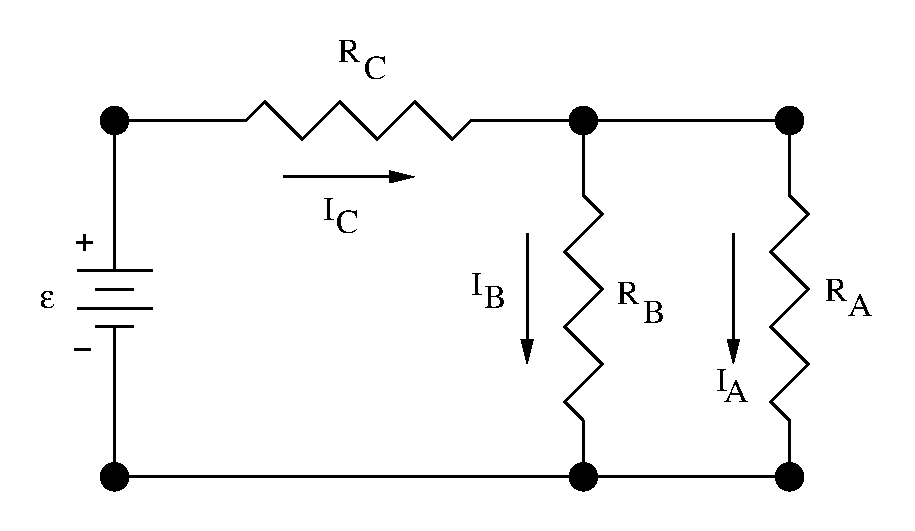
\includegraphics{kirchhoffs_rules/kirchhoffs_rules_fig_1.eps}} \par}
\vspace{0.3cm}

\begin{enumerate}
\item Referring to the circuit above, choose a junction and write an equation
which satisfies Kirchhoff's first rule.\vspace{20mm}

\item Identify two closed loops on the circuit which contain at least one
element not included in the other. Write an equation for each loop
that satisfies Kirchhoff's second rule.\vspace{20mm}

\item You now have three equations that can be solved for the three currents
in terms of the supplied voltage (emf), \( \varepsilon  \), and the
three resistors, R\( _{A} \), R\( _{B} \), and R\( _{C} \). Carry
out the algebra to obtain expressions for the three currents in terms
of these quantities.\vspace{50mm}

\item Now use Ohm's law and the sum rules for resistors in series and in
parallel to derive expressions for the three currents.\vspace{50mm}

\item Are the results of 3 and 4 the same? They should be.\vspace{15mm}

\item Set a digital multimeter to measure resistance. Determine and record
values for the three resistors, R\( _{A} \), R\( _{B} \), and R\( _{C} \),
which are mounted on the wooden block.\vspace{15mm}

\item \textbf{Prediction}: if the emf, \( \varepsilon  \), were 5.0 V,
what do you predict the three currents would be?\vspace{30mm}

\item Configure the circuit as in the figure above, using the power supply
as the source of emf. With the power supply off, set the current control
at mid-range and the voltage control all the way down. Set the digital
multimeter to measure voltage and connect it in parallel with the
power supply to measure \( \varepsilon  \). Connect the analog ammeter
in series with resister R\( _{A} \) to measure the current I\( _{A} \).
\item After checking with your instructor that the circuit is correct, turn
on the power supply and set \( \varepsilon  \) to about 5.0 V. Record \( \varepsilon  \) and I\( _{A} \), then turn off the power supply.\vspace{15mm}

\item Set up the circuit to measure I\( _{B} \). After getting assurance
from you instructor that your circuit is correct, turn on the power
supply and record \( \varepsilon  \) and I\( _{B} \). Turn off the
power supply.\vspace{15mm}

\item Set up, measure and record I\( _{C} \).\vspace{15mm}

\item Do your results agree with your prediction? How large, in terms of
percentage, are the discrepancies? Speculate on what might cause any
differences.\vspace{15mm}
\end{enumerate}

